\section{High-level languages and tools}
\label{sec:tools}

To design complex digital circuits, tools for reduction and management
of complexity is needed. Usually, the designer expres the behaviour of
circuits in a hardware description language (HDL), which provides an
abstraction over the underlying hardware. While ordinary design tools
and languages, such as VHDL and Verilog, are not usually used to
synthesize clockless circuits, there is not an inherent limitation in
the languages that prevents this as demonstrated in
\cite[pp. 135-137]{sparso}.

Much of the work on high-level modeling and synthesis of clockless
circuits is based on the CSP language paradigm. The CSP language,
``Communicating Sequential Process'' was proposed by Hoare \cite{csp},
and is based on the mathematical theories of concurrency from process
algebra. CSP-languages allows concurrent processes, composition of
both sequential and parallel statements within a process, and
synchronous message passing between the processes.

\begin{figure}[htbp]
  \centering
  \includegraphics{tangtool.pdf}
  \caption{Tangram design flow. Figure from \cite{fullscan}. XXX compare to TiDE}
  \label{fig:tangtool}
\end{figure}

XXX Null convention logic


Tangram is a high-level language in the CSP family, introduced by
Philips in 1991 to define clockless circuits. The Tangram compiler
generates what is referred to as handshake circuits, and has its own
toolset and workflow as illustrated in
Figure~\ref{fig:tangtool}. Tangram was later transferred from Philips
to the company Handshake Solutions, and the name of Tangram was
changed to Haste. As of this writing, Haste has entered a state of
maintenance, and has been readsorbed into Philips.

\begin{figure}[htbp]
  \centering
  \includegraphics{handbuffer.pdf}
  \caption{Handshake buffer a) defined in Balsa source code and b)
    implemented as a handshake circuit. Figure from
    \cite{taylor2008automatic}.}
  \label{fig:handbuffer}
\end{figure}

Handshake circuits, first described in \cite{12, teakxxx}, consists of
40 different basic components that can be connected by four-phase
handshake signalling. The components has active and passive ports,
where the active components initiates the handshake and is said to
``push'' the data. Figure~\ref{fig:handbuffer}.b illustrates a
handshake circuit for a one-place buffer. Active ports are denoted
with a filled circle.

To map handshake-circuits to hardware, the handshake components are
replaced by their gate-level equivalents, depending on implementation
style. Implementation styles can be bundled data, QDI, or even clocked
for e.g. verification on conventional FPGAs. Tangram is also a so
called syntax-directed language, meaning that each language construct
is deterministically mapped to a handshake-component. This allows the
designer to better understand and optimize circuits as they are
written.


There are multiple circuits implemented in Tangram/Haste. XXX list and
explain different circuits.

Balsa is another CSP-like language based on the priciples from Tangram,
and is an attempt to define a more expressive language. Balsa also
introduces a intermediate file format, breeze, which contains the
netlist for the handshake components. Breeze can later be implemented
into standard-cell logic by. Figure~\ref{fig:balsatool} shows Balsa
and it's related tools.

Tangram and Balsa are referred to as being a ``syntax-directed''
languages. This means that the silicon compiler transparently and
predictably generates components from each language construct. In
Figure~\ref{fig:handbuffer} it is shown how a simple Balsa-program is
translated into a handshake circuit. Each language-construct, loop,
sequence, transfer, and variable, are translated into handshake
components on a one-to-one basis.

Balsa has for example been used to implement two major circuits: The
DMA-controller for the Amulet3a processor, and the ARM-compatible SPA
processor itself. Balsa is released to the public domain under the
GPLv2 licence.

Handshake component based designs has been shown to use little power,
but also to have low performance \cite{80c51}. Handshake-circuits
exhibit a control heavy structure which inhibits performace. Teak
\cite{teak} introduces a new target component set and synthesis scheme
for synthesizing Balsa circuits as an attempt to mitigate this
drawback. Instead of focusing on control

While Balsa-circuits consists of capacity-less channels, where data on
the channel has to be valid from request to acknowledge, Teak allows
buffers to be automatically inserted into the dataflow, allowing
decoupling. 

Teak circuits have been demonstrated to exhibit 4.6\% to 18.39\% worse
performance than Balsa-circuits when syntehsizing to a fixed gate
delay dual-rail four-phase implementation. However, Teak has a larger
headroom for automated optimising transformations.

\subsection{Testing XXX:remove this}


Clockless circuits usually uses latches and C-elements for
memory. These memory-elements are not directly scanable, and they are
not connected to any global clock. However, in \cite{fullscan}, it is
shown how Tangram compiled, clockless circuits can be made scanable by
replacing all state-holding handshake components with scanable
equivalents. In Figure~\ref{scanC}, from \cite{fullscan}, a scanable
C-element is shown. These components are then connected into a serial
scan chain which is compatible with existing ATPG tools.

It is important to note that the scan-chain insertion is done at the
technology-mapping stage, allowing the designer to insert test-logic
into the library of components. For Balsa and Teak, this will require
some modifications of the compilers to chain the memory elements
together into a scan chain, and to provide a global testing clock.

As the testing is done synchronously, it also means that a global
clock have to be implemented. However, this clock has more relaxed
requirements than that of an clocked circuit, since the clock used for
testing runs at lower speeds than the circuit itself is capable of.

\section{new tool}


Languages such as Verilog and VHDL are used to model and simulate
behaviour of digital circuits, and while not all Verilog and VHDL
programs can be synthetizised, a well defined subset can.

Clocked circuits are often expressed in theese languages, but there is
nothing inherent in the languages that prevent a designer from
expressing a clockless circuit. In fact, methods for this have been
used in XXX. However, as shown in \cite[pp XXX]{sparso}, this is
rather cumbersome, and most of the work done on HDLs for clockless
circuits are founded on the programming paradigm introduced with the
language Communicating Sequentaial Processes (CSP)\cite{xxx}, based on
mathematical foundations from process algebra.

As the name partly implies, CSP is baesd on connecting many processes
together whith handshake channels. The most known language based on
CSP is Tangram, designed in 1991 by Philips. Tangram was later split
out to its own company, and changed name to Hast due to trademarking
issues. Haste has now been readsorbed into Philips.

Tangram was used to create multiple circuiots: A XXX microprocessor,
low power smart card XXX, and showed the practical strengths of the
language, design tools,  and clockless circuit design as a
whole.

Tangram emits handshake circuits, first described in
\cite{12,teakxxx}, based on a library of around 40 handshake
components, whith some of theese shown in
figure~\ref{fig:hs}. Figure~\ref{fig:hsbuf} show an one-place buffer
handshake circuit, whith the explicit equest and acknowledge signals
drawn on top. To implement such circuits to hardware, the handshake
components are replaced with their gate-level equivalents, depending
on implementation style. Implementation styles can be bundled data,
QDI, or even clocked for e.g. verification on conventional FPGAs.


To facilitate further research on clockless circuits whithin the
CSP-paradigm, the language ``Balsa'' was designed at Manchester
University \cite{xxx}, and released to the public domain under a GPLv2
license \cite{gpl}. The most complex circuit designed with the balsa
tools, is a clockless ARM\cite{arm} compatible CPU\cite{spa}.

Research have shown that handshake circuits uses little power\cite{xxx},
but also exhibits poor performance\cite{xxx}. Work has been done to
alleviate this\cite{xxx}, but the performance is still rougly half of
clocked equivalents.

To explore and facilitate experiments with automatic optimizations,
and to create more data-flow oriented circuits, ``Teak''\cite{teak}
was recently created, compiling Balsa-programs to a reduced set of 8
different teak-compontents. Teak currently performs worse than the
more mature synthesis tools, but have more room for experimentation
and improvement at the compiler level.


